\section{Resultados}

\subsection{Estructura técnica y verificación de integridad criptográfica}
La lectura inicial del archivo \texttt{data/persona.csv} mediante análisis de flujo determinó la perfecta coherencia estructural de la matriz de datos: no se encontraron encabezados duplicados, líneas incompletas ni anomalías de delimitación. En la tabla \ref{tab:estructura} se resumen las métricas básicas de integridad observadas en la copia original.

\begin{table}[htbp]
\centering
\caption{Características estructurales y verificación del archivo de entrada}
\label{tab:estructura}
\begin{tabularx}{0.88\textwidth}{Xr}
\toprule
\textbf{Parámetro de control} & \textbf{Resultado observado} \\
\midrule
Registros totales de personas ($N$) & 39.497 \\
Hogares únicos identificados ($N_{\text{hog}}$ vía \texttt{folio}) & 12.718 \\
Atributos / Columnas & 275 \\
Volumen en disco & 34.568.646 bytes \\
Codificación de caracteres & UTF-8 sin BOM \\
Encabezados duplicados o corruptos & 0 \\
Registros con anchura de campos incorrecta & 0 \\
Filas idénticas repetidas en la matriz & 0 \\
Claves primarias candidatas \texttt{(folio, nro)} duplicadas & 0 \\
\bottomrule
\end{tabularx}
\par\vspace{3pt}\parbox{0.88\textwidth}{\footnotesize\textit{Nota.} SHA-256: {\scriptsize\texttt{568e82e3039d991a1ee0d8e2056448f8c465c03ffa838330c4f1522dd77bddc8}}. Fuente: Manifiesto de ejecución local.}
\end{table}

\subsection{Diagnóstico de ausencias y refutación del descarte ciego (L-80)}
El diagnóstico cuantitativo sobre las 10.861.675 celdas del dataset reveló la presencia de 771.655 celdas exactamente vacías (\texttt{""}), 5.489.754 tokens explícitos de no respuesta (\texttt{NA}) y 1.192.066 celdas con el valor numérico legítimo \texttt{0}. 

Tal como se ilustra en la figura \ref{fig:diagnostico_ausencia} (Panel A), los tokens \texttt{NA} representan el 50,5\% de las celdas totales. Sin embargo, este volumen no traduce una mala calidad de recolección, sino la existencia de módulos del cuestionario con saltos condicionales. En una corrida preliminar histórica, la aplicación de una regla ciega de umbral al 80\% (L-80 calculada sobre todas las filas) excluyó indebidamente 125 variables. Como se demuestra en el Panel B de la figura \ref{fig:diagnostico_ausencia}, la variable de salario líquido (\texttt{s04c\_17a}) presenta 81,35\% de ausencia en la población global, pero al delimitar su universo real a las personas asalariadas elegibles ($N = 7.370$), solo 4 casos corresponden a faltantes reales (0,05\% de omisión). Por ello, el maestro definitivo retiene la totalidad de las 275 variables.

\begin{figure}[htbp]
\centering
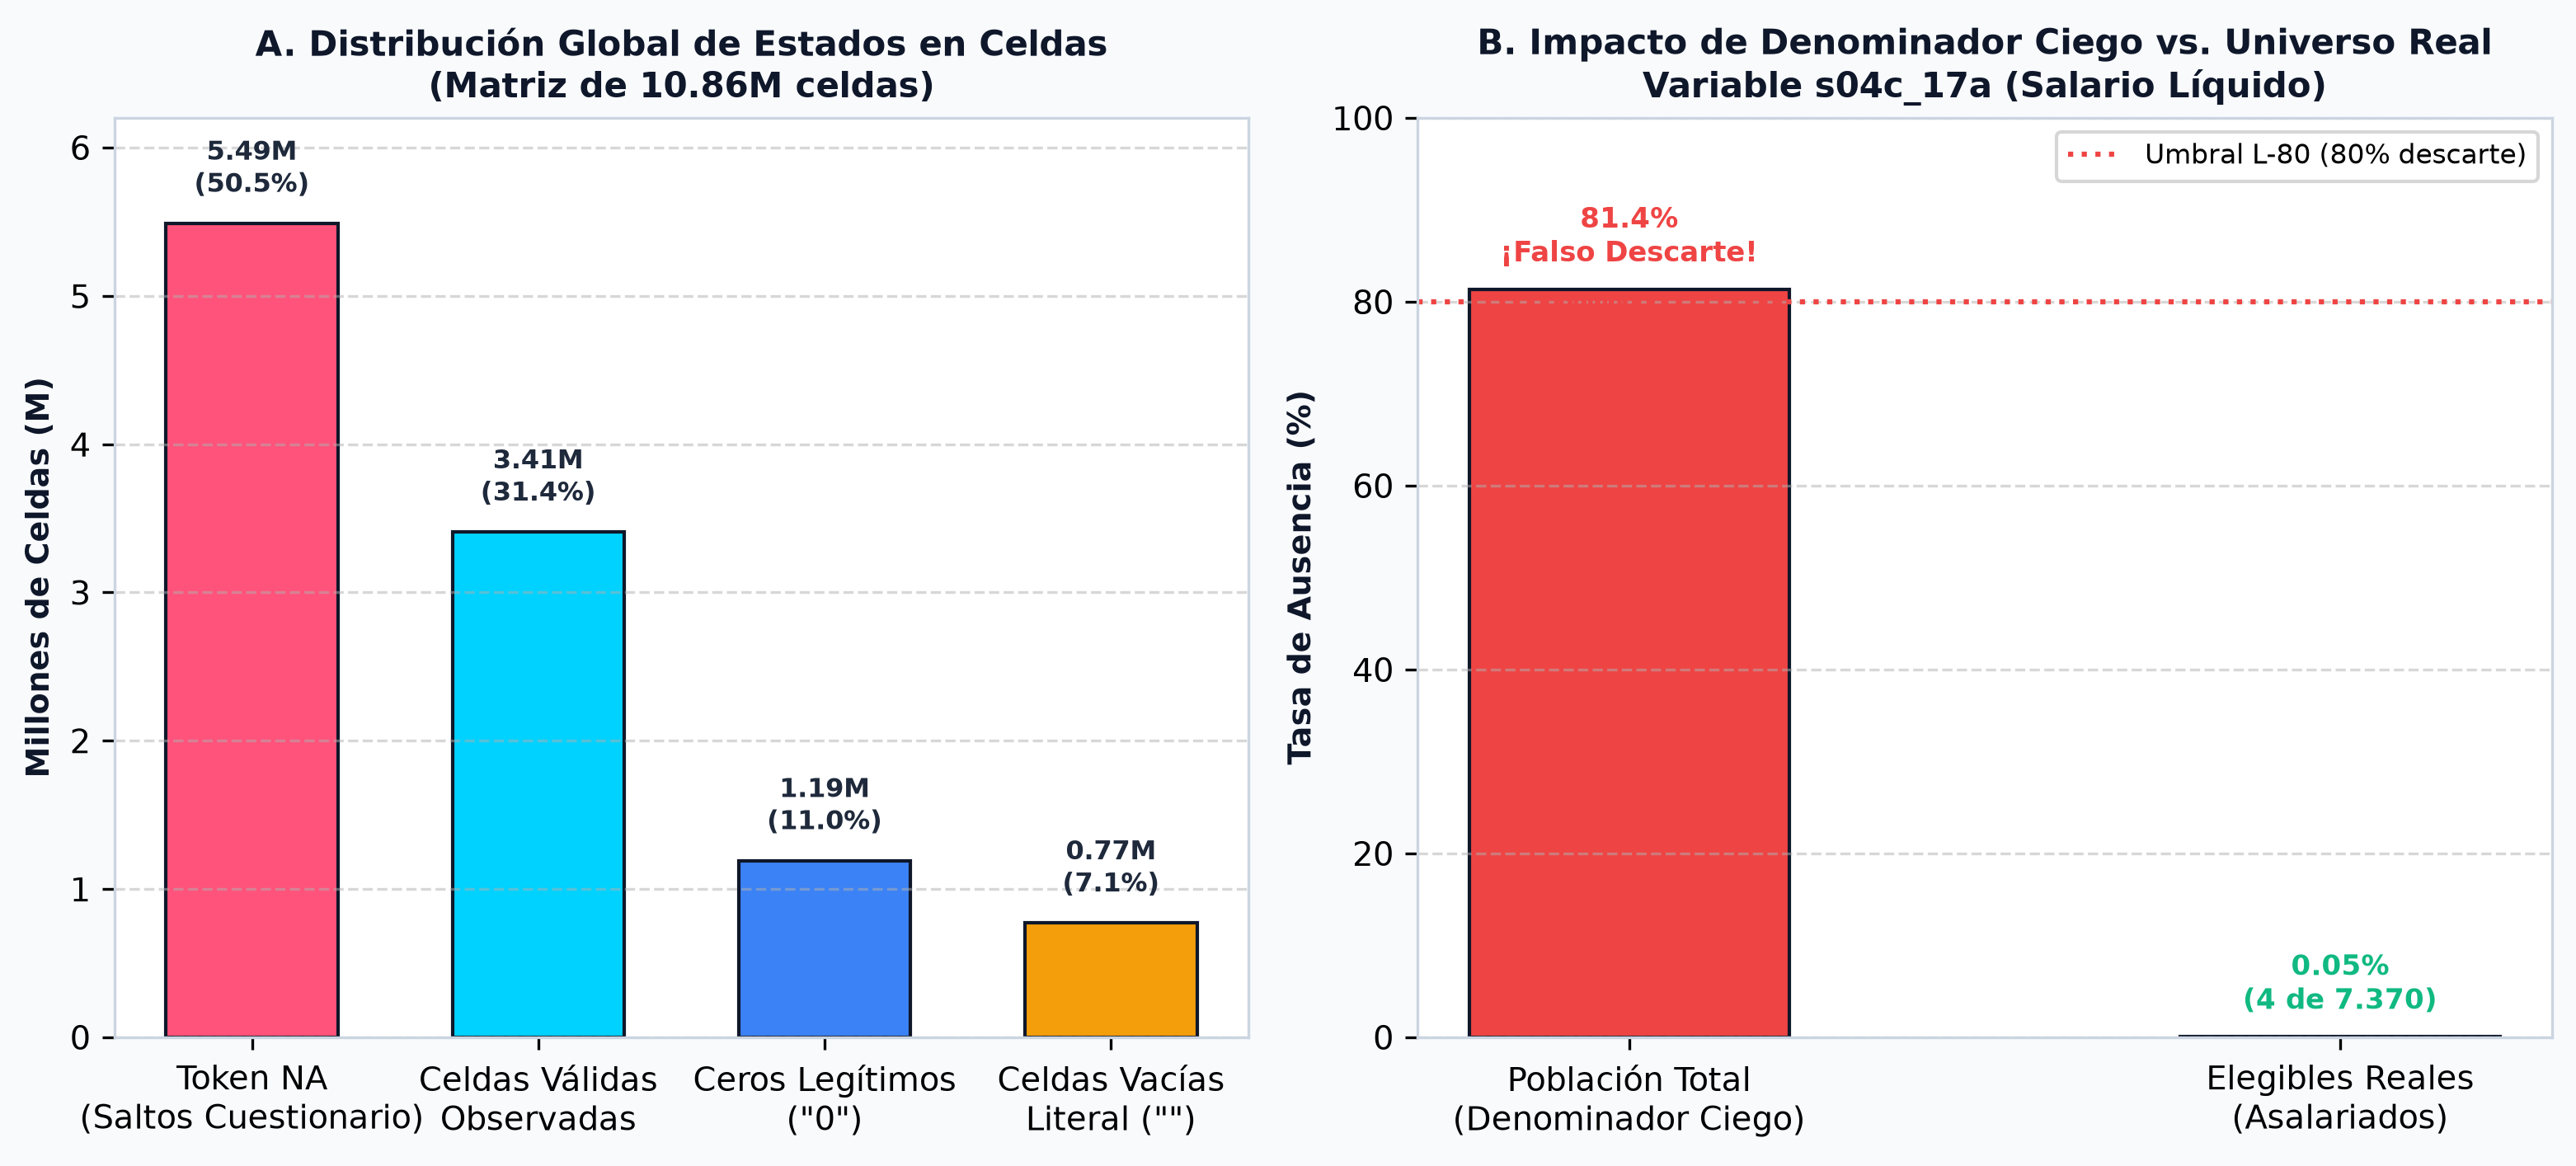
\includegraphics[width=0.98\textwidth]{figuras/fig3_diagnostico_tokens_ausencia.png}
\caption{Diagnóstico de estados de ausencia en celdas y falacia del descarte global por L-80}
\label{fig:diagnostico_ausencia}
\par\vspace{3pt}\parbox{0.98\textwidth}{\footnotesize\textit{Nota.} El panel A clasifica los 10,86 millones de celdas. El panel B demuestra cómo el 81,4\% de ausencia en salario líquido (\texttt{s04c\_17a}) se reduce a 0,05\% al evaluarse en su población elegible documentada.}
\end{figure}

\subsection{Catálogo de reglas de calidad y transformaciones trazadas}
La versión definitiva de trabajo, identificada como \texttt{\small persona-\allowbreak 317279aa\allowbreak fe9023a2}, mantiene la totalidad de los 39.497 registros y las 275 columnas tanto en formato CSV como en Apache Parquet. En la tabla \ref{tab:reglas} se sintetiza el impacto medible de cada regla de limpieza aplicada.

\begin{table}[htbp]
\centering
\caption{Catálogo consolidado de reglas de preparación y limpieza ejecutadas}
\label{tab:reglas}
\begin{tabularx}{\textwidth}{>{\raggedright\arraybackslash\small}p{1.2cm}>{\raggedright\arraybackslash\small}p{3.8cm}>{\raggedright\arraybackslash\small}p{1.7cm}>{\raggedright\arraybackslash\small}X}
\toprule
\textbf{Regla} & \textbf{Condición y fundamento} & \textbf{Impacto real} & \textbf{Efecto analítico y evidencia} \\
\midrule
\textbf{L-01} & \texttt{(folio, nro)} como clave compuesta tipada a enteros $\mathbb{Z}^+$. & 39.497 tuplas verificadas & Cero colisiones; confirma estructura de hogar y persona. \\
\textbf{L-02} & Taxonomía diferenciada entre vacío, token \texttt{NA} y cero legítimo. & 7,45M celdas clasificadas & Preservación de saltos; prohibición de imputación ciega con medias. \\
\textbf{L-03} & Trim de espacios blancos en 256 columnas numéricas y códigos. & 256 columnas normalizadas & Estandarización de tipos en Parquet sin afectar texto libre. \\
\textbf{L-04} & Verificación de códigos contra catálogo oficial DDI F27 del INE. & 100\% de conformidad & Validación de \texttt{depto} (1..9), \texttt{area} (1,2) y \texttt{s01a\_01} (1,2). \\
\textbf{S-01} & Frontera física biológica: horas semanales $\le 168$ ($7 \times 24$). & 3 celdas tratadas a \texttt{NA} & Corrección en \texttt{phrs}, \texttt{shrs}, \texttt{tothrs} (171.5h, 180h y 192h). Filas conservadas. \\
\textbf{S-02} & Normalización a minúsculas solo en texto abierto de especificación. & 12.516 celdas corregidas & Aplicada en 13 columnas específicas; claves y códigos intactos. \\
\textbf{L-80} & Monitoreo de alta ausencia técnica global ($>80\%$). & Alerta informativa & Prohíbe descarte destructivo; variables conservadas en el maestro. \\
\bottomrule
\end{tabularx}
\par\vspace{3pt}\parbox{\textwidth}{\footnotesize\textit{Nota.} El archivo maestro resultante conserva el 100\% de filas y atributos originales. Las alteraciones semánticas de la regla S-01 están registradas en \texttt{semantic\_cell\_changes\_restricted.csv}.}
\end{table}

La regla S-01 se detalla en la figura \ref{fig:auditoria_s01}: se contrastó la distribución de jornadas laborales con el límite biológico semanal, registrándose en bitácora auditable la reasignación de las 3 celdas físicamente anómalas.

\begin{figure}[htbp]
\centering
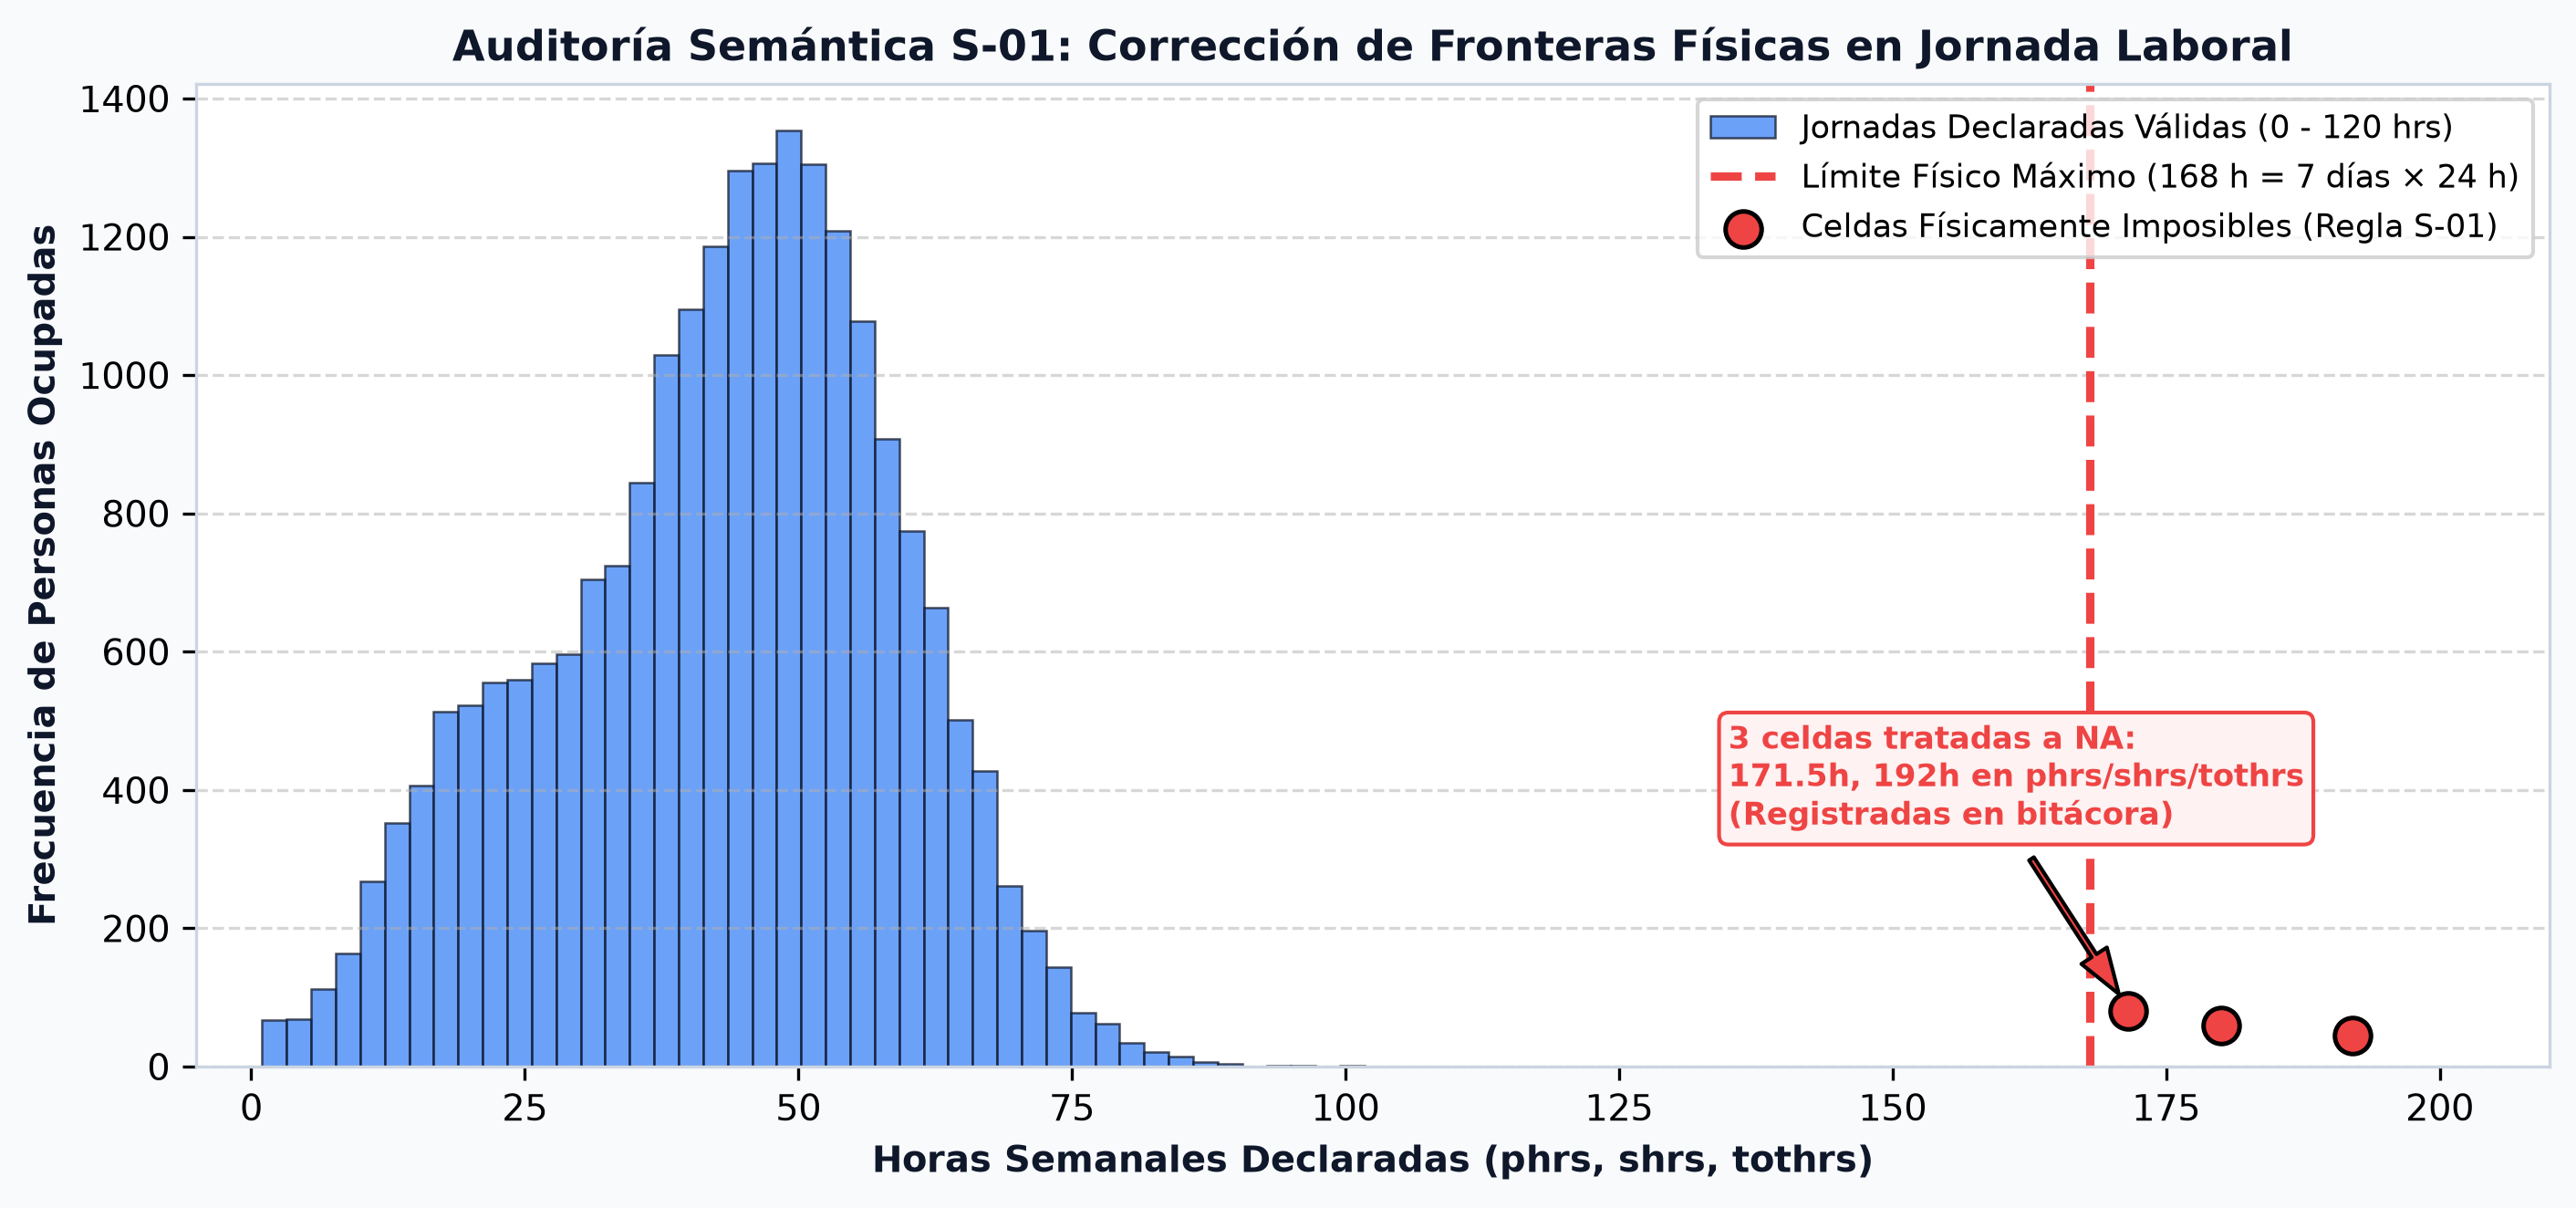
\includegraphics[width=0.92\textwidth]{figuras/fig5_auditoria_horas_semanales_s01.png}
\caption{Auditoría semántica de la regla S-01: Control de límites físicos en jornada semanal}
\label{fig:auditoria_s01}
\par\vspace{3pt}\parbox{0.92\textwidth}{\footnotesize\textit{Nota.} Distribución de horas semanales declaradas y reasignación trazable de los valores extremos imposibles ($> 168$ h) sin eliminación de observaciones.}
\end{figure}

\subsection{Delimitación territorial de la muestra por departamento}
La distribución espacial observada de los 39.497 encuestados refleja la cobertura del operativo censal en los nueve departamentos de Bolivia. En la figura \ref{fig:distribucion_departamental} se presenta el desglose según área urbana y rural. Se advierte una alta concentración urbana en los departamentos del eje central (La Paz con 86,1\%, Santa Cruz con 88,5\% y Cochabamba con 82,0\%), frente a una predominancia rural acentuada en Potosí (40,5\%) y Chuquisaca (31,5\%).

\begin{figure}[htbp]
\centering
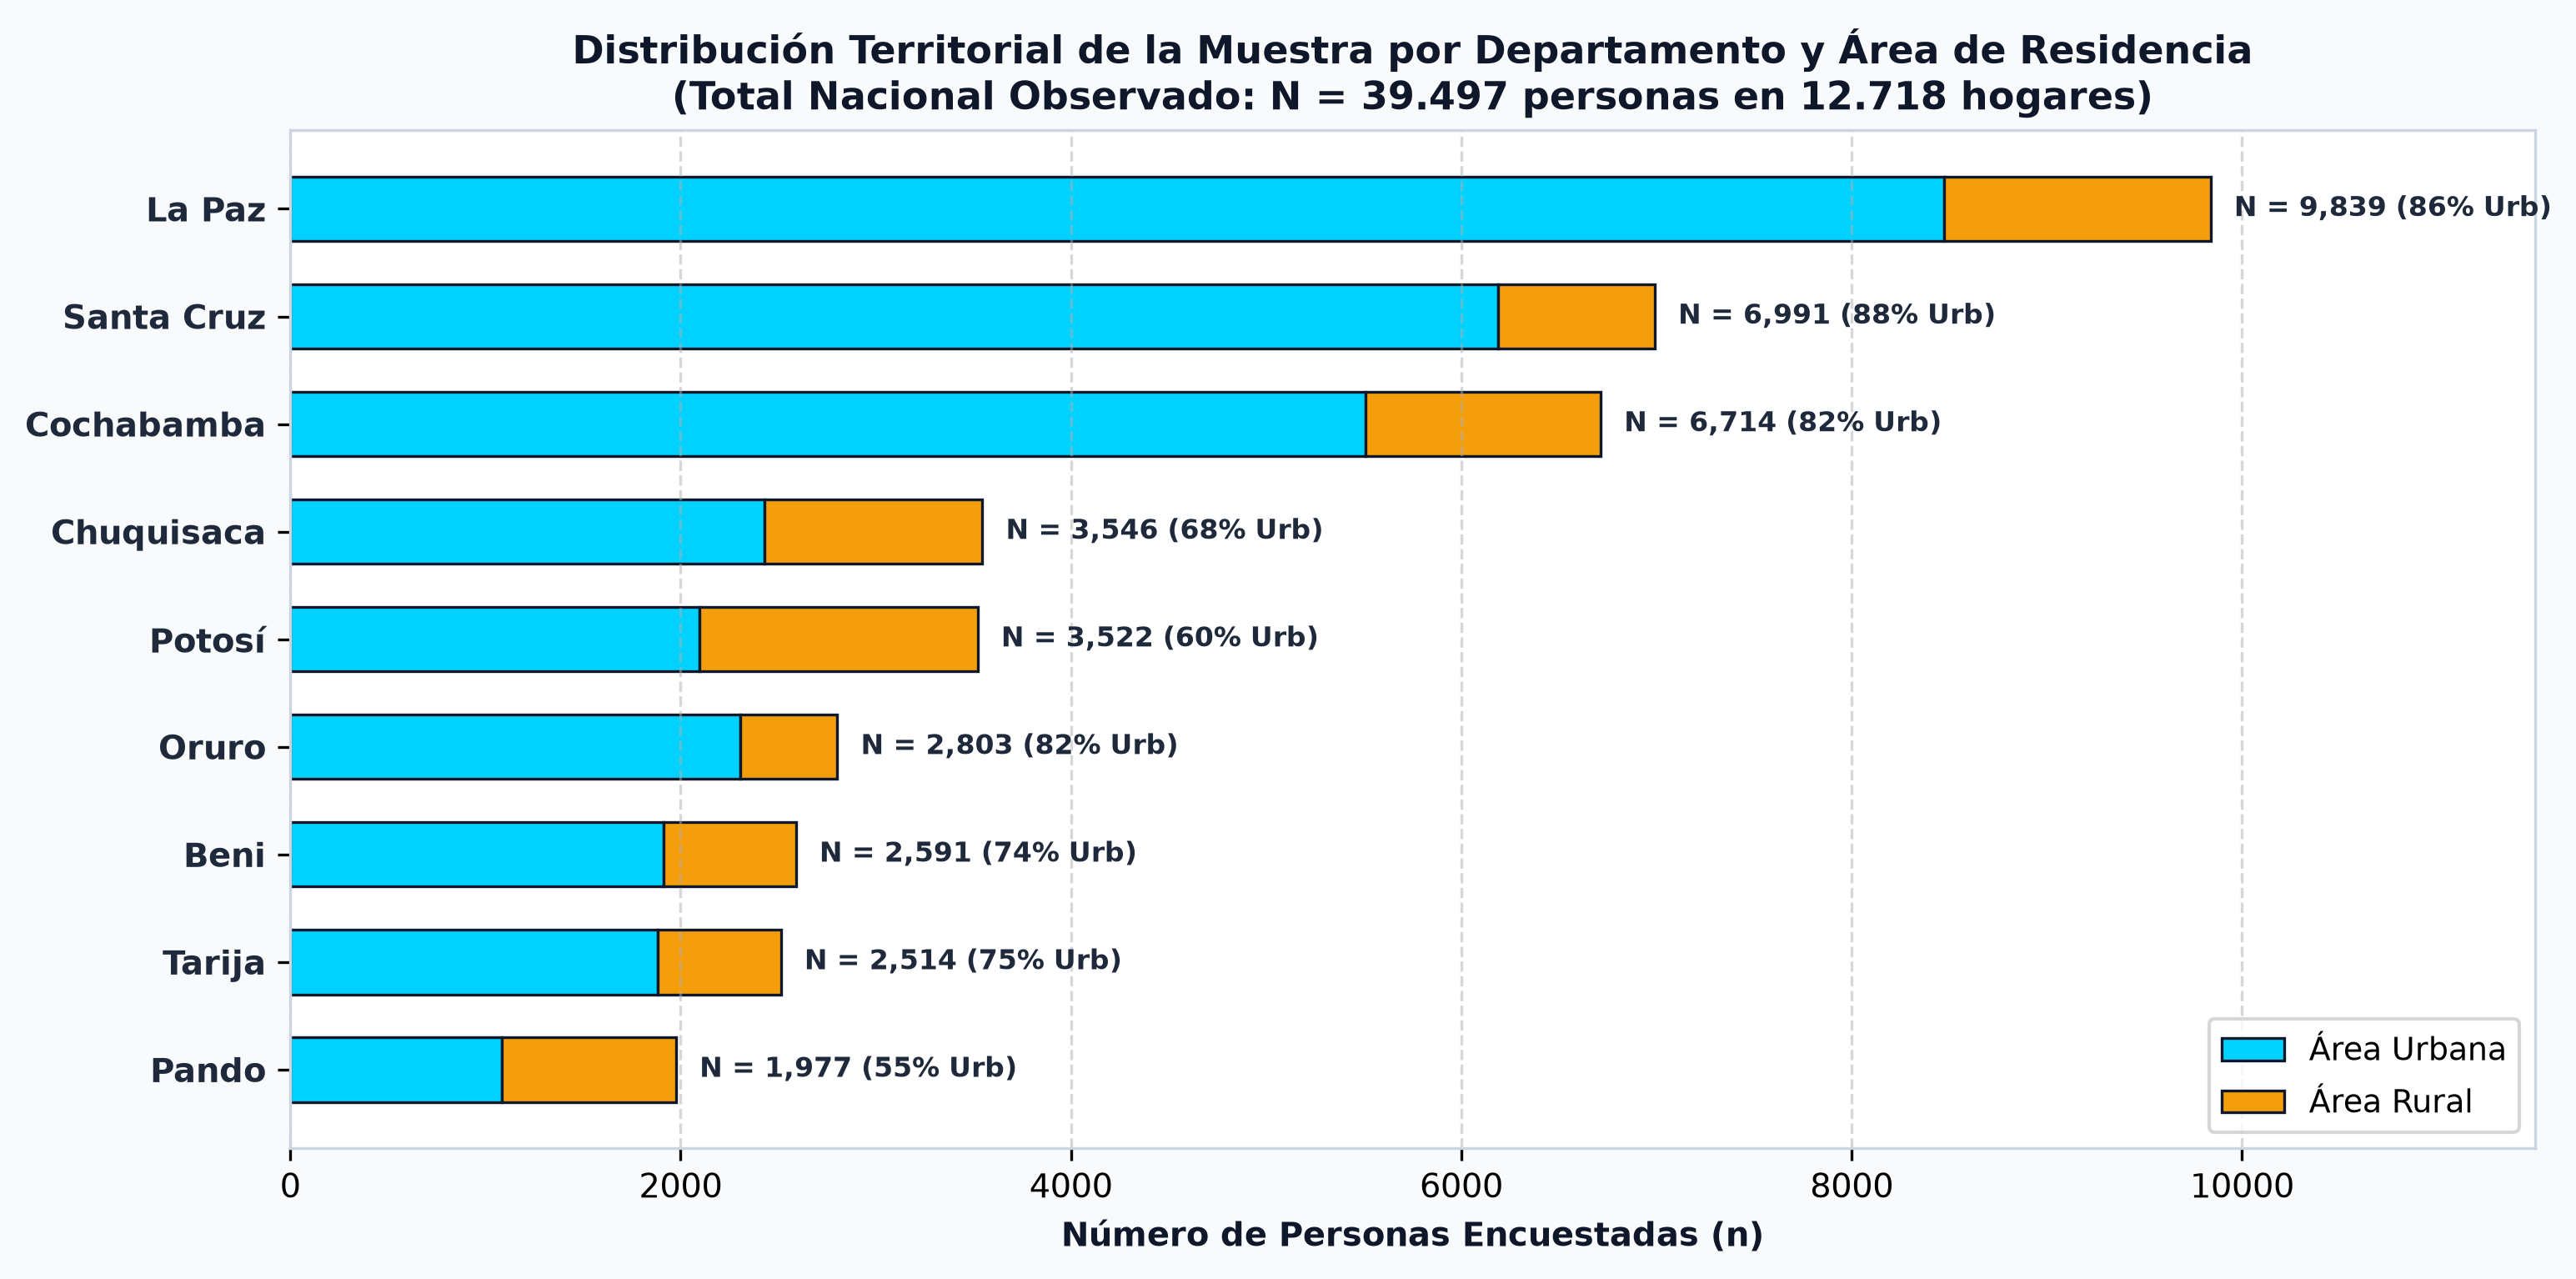
\includegraphics[width=0.98\textwidth]{figuras/fig4_distribucion_departamental.png}
\caption{Distribución territorial observada de la muestra por departamento y área de residencia}
\label{fig:distribucion_departamental}
\par\vspace{3pt}\parbox{0.98\textwidth}{\footnotesize\textit{Nota.} Conteo de registros válidos por departamento desagregados en área urbana y rural ($N = 39.497$ personas y $N_{\text{hog}} = 12.718$ hogares).}
\end{figure}

\subsection{Segmentación analítica: Las 11 vistas temáticas}
Para resolver el dilema entre conservar las 275 variables maestras y facilitar consultas estadísticas sobre subpoblaciones específicas, se derivaron 11 vistas temáticas no destructivas, alojadas en el subdirectorio \texttt{thematic\_views/} y sincronizadas mediante \texttt{views\_manifest.json}. La especificación formal de cada vista se presenta en la tabla \ref{tab:vistas_tematicas} y su cobertura comparativa en la figura \ref{fig:cobertura_vistas}.

\begin{table}[htbp]
\centering
\caption{Especificación técnica y criterios de elegibilidad de las 11 vistas temáticas}
\label{tab:vistas_tematicas}
\begin{tabularx}{\textwidth}{>{\raggedright\arraybackslash\small}p{2.85cm}>{\raggedright\arraybackslash\small}p{4.35cm}>{\raggedleft\arraybackslash\small}p{1.2cm}>{\raggedleft\arraybackslash\small}p{1.1cm}>{\raggedright\arraybackslash\small}X}
\toprule
\textbf{Identificador} & \textbf{Criterio / Filtro de elegibilidad oficial} & \textbf{Filas ($n$)} & \textbf{Cols} & \textbf{Universo de análisis} \\
\midrule
\texttt{\small demografia} & Muestra completa sin filtro restrictivo & 39.497 & 33 & Sociodemográfico general \\
\texttt{\small salud\_general} & Toda persona encuestada & 39.497 & 31 & Afiliación y centros \\
\texttt{\small salud\_fecund} & Mujeres de 13 a 50 años (\texttt{\small s01a\_02=2}) & 11.328 & 24 & Maternidad e historial \\
\texttt{\small salud\_infant} & Menores de 6 años de edad (\texttt{\small edad < 6}) & 3.434 & 10 & Desarrollo infantil \\
\texttt{\small salud\_bono} & Menores de 5 años de edad (\texttt{\small edad < 5}) & 2.781 & 12 & Vacunas y Bono Juana Azurduy \\
\texttt{\small educacion} & Población de 4 años o más (\texttt{\small edad $\ge$ 4}) & 37.354 & 43 & Asistencia y alfabetismo \\
\texttt{\small empleo\_pet} & Población en Edad de Trabajar (\texttt{\small edad $\ge$ 7}) & 35.366 & 121 & Actividad y ramas \\
\texttt{\small empleo\_sec} & Ocupados con 2do trabajo (\texttt{\small s04e\_25=1}) & 1.357 & 45 & Jornada secundaria \\
\texttt{\small ingresos\_nolab}& Todos los registros persona & 39.497 & 48 & Jubilaciones y bonos \\
\texttt{\small ingresos\_pob} & Todos los registros persona & 39.497 & 25 & Pobreza y per cápita \\
\texttt{\small hogar\_resumen} & Un registro por vivienda única (\texttt{\small folio}) & 12.718 & 18 & Agregados del hogar \\
\bottomrule
\end{tabularx}
\par\vspace{3pt}\parbox{\textwidth}{\footnotesize\textit{Nota.} La vista de hogar consolida variables invariantes por vivienda resolviendo ausencias sin colisión de valores observados. Fuente: \texttt{views\_manifest.json}.}
\end{table}

\begin{figure}[htbp]
\centering
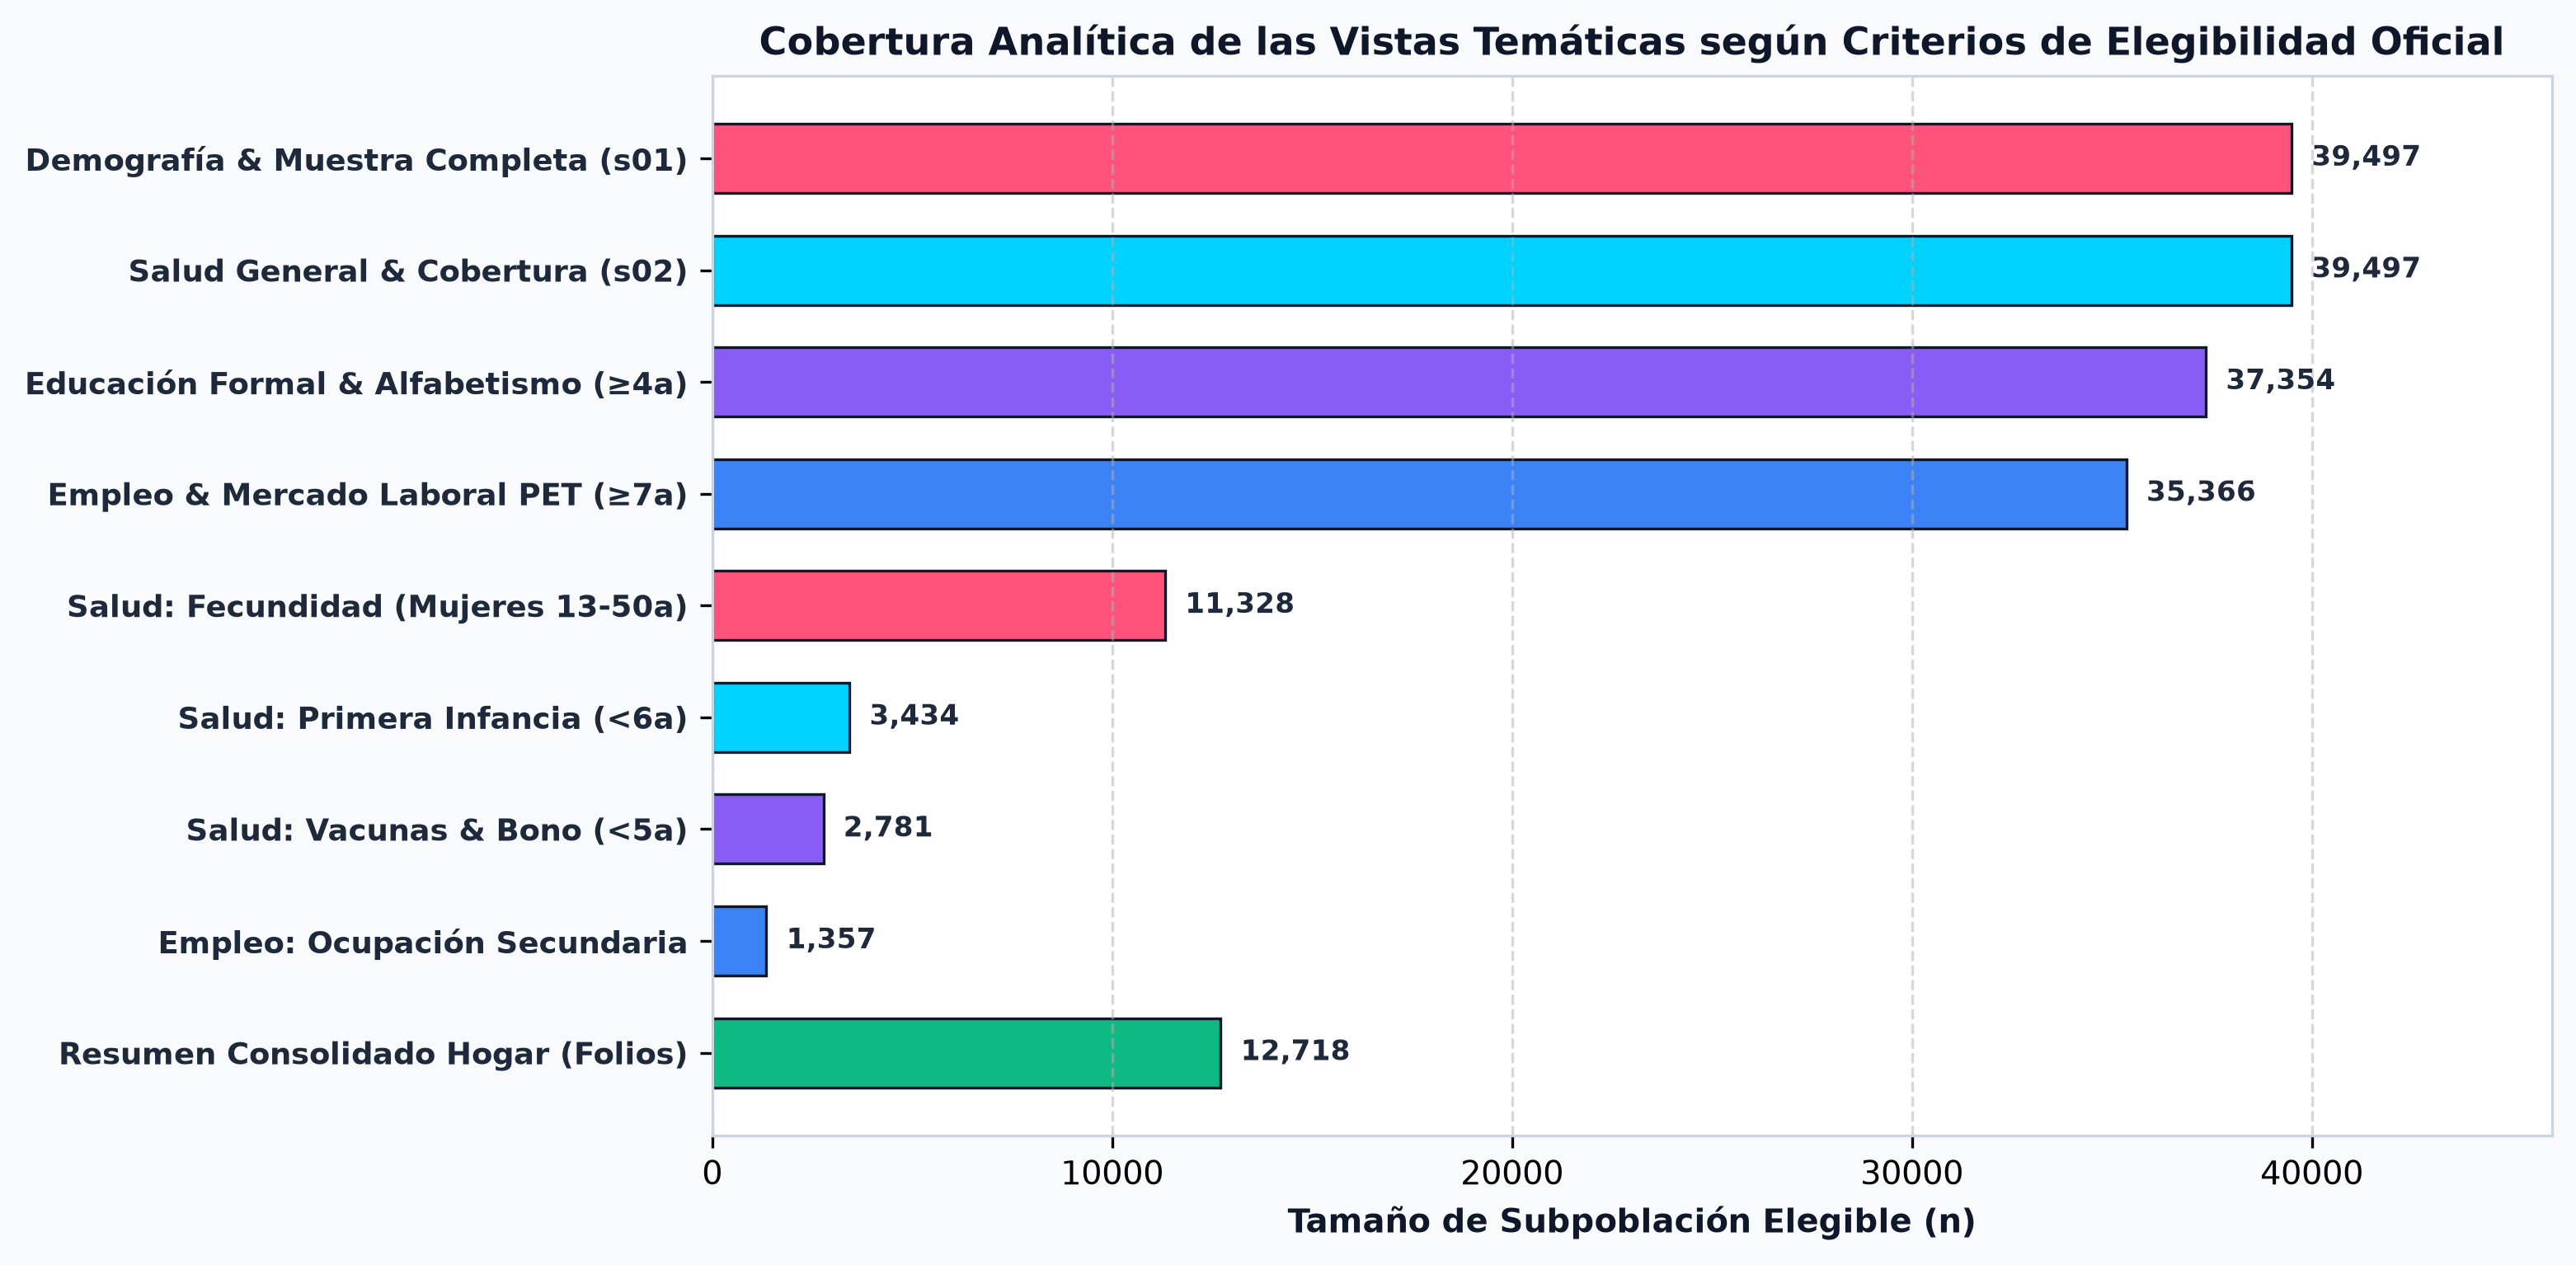
\includegraphics[width=0.98\textwidth]{figuras/fig6_cobertura_11_vistas.png}
\caption{Población elegible y cobertura analítica de las 11 vistas temáticas}
\label{fig:cobertura_vistas}
\par\vspace{3pt}\parbox{0.98\textwidth}{\footnotesize\textit{Nota.} Comparativa del tamaño muestral ($n$) retenido en cada módulo de acuerdo con los filtros de salto del cuestionario.}
\end{figure}

\subsection{Auditoría intrahogar en la muestra de control (QA)}
En la muestra determinista de control de 381 hogares (1.216 integrantes), se auditó la coherencia entre el número de personas observadas en el archivo y la variable declarada \texttt{totper}. Se constató que \texttt{totper} coincidió con las filas observadas en 69 hogares y registró diferencias en 312 casos. Al tratarse de una extensión local no documentada en el catálogo F27 del INE, se mantuvo intacta y no se utilizó como denominador en cálculos poblacionales, documentando la discrepancia en el registro de incidencias del catálogo.
